%Preamble
% Some of these are recommended by "9 LaTeX packages everyone should use" http://www.howtotex.com/packages/9-essential-latex-packages-everyone-should-use/, 
%others were added as I came across the need for them.



\documentclass[a4paper,12pt,fleqn]{article}
\setlength{\parindent}{0em}
\usepackage{amsmath}
\usepackage{fancyhdr}
\usepackage{siunitx}
\usepackage{enumitem}
\usepackage{amsmath}
\usepackage{graphicx}
\usepackage{tikz}
\usepackage{import}
\usepackage{comment}
\usepackage[table, usenames, dvipsnames]{xcolor}
\definecolor{lightgray}{gray}{0.9} % I used this for the table background colour
\usepackage{multirow} % needed if cells in a table need to span more than one row
\usepackage{tabu} % makes table columns all have the same width
\usepackage[
backend=biber,
style=authoryear,
sorting=ynt
]{biblatex} % needed for citations and references

% Unit definitions %%%%%%%%%%%%%%%%%%%%%%%%%%%%%%%%%%

\DeclareSIUnit\kilowatthour{kWh}
\DeclareSIUnit\kilowattpeak{kW_P}
\DeclareSIUnit\kVA{kVA}
\DeclareSIUnit\kVAR{kVAR}
\DeclareSIUnit\year{y}
\DeclareSIUnit\north{N}
\DeclareSIUnit\south{S}
\DeclareSIUnit\second{s}
\usepackage{cleveref}
\usepackage{exercise} % does all the things with exercises and solutions.

%\\\\\\\\\\\\\\\\\\\\\\\\\\\\\\\\\\\\\\\\\\\\\\\\\\\\\\\\\\\\\\\\\\\\\\\\\\\\\\\\\\\\\\\\\\\\\\\\\\\\\\\\\\\\\\\\\\\\\\\\\\\\\\\\\\\\\\

\begin{document}

% Title stuff
\title{The Geothermal Resource}
\author{Michael Hunt}
\date{}
\maketitle

%\\\\\\\\\\\\\\\\\\\\\\\\\\\\\\\\\\\\\\\\\\\\\\\\\\\\\\\\\\\\\\\\\\\\\\\\\\\\\\\\\\\\\\\\\\\\\\\\\\\\\\\\\\\\\\\\\\\\\\\\\\\\\\\\\\\\\\
\begin{figure}[h]
\centering
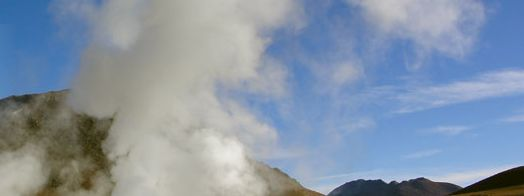
\includegraphics[width=1.0\textwidth]{./figures/SteamGeysers}
\caption{Steam geysers at Yellowstone Park}
\end{figure}

\section{Introduction}
This is a very brief introduction to the field of geothermal energy. More comprehensive information can be found in \cite{Press1986} and \cite{Fowler2005}\\
Geothermal energy is heat derived from a few km underground, where it is hotter than the surface of the earth for three reasons:
\begin{enumerate}
\item Heat flowing through to the mantle and hence to the crust from the earth's core, which is much hotter still, despite having been cooling down since the earth was created several billion years ago.
\item Tidal friction in the core of the earth.
\item Radioactive decay in the crust and mantle of the earth. This accounts for about 80\% of the heat flux.
\end{enumerate}
\begin{table}
\caption{The distribution of radioactive isotopes within rock type fund within the crust (granite, basalt) and the mantle (peridotite). Clearly, the crust has a far higher proportion of these than the mantle}
\begingroup\setlength{\fboxsep}{0pt}
\colorbox{lightgray}{%
\begin{tabu} { | X[c] | X[c] | X[c] | X[c] | X[c] | }
\hline
\multirow{3}{*}{\textbf{Rock type}} & \multicolumn{3}{| c |}{\textbf{Abundance within rock type / ppm}}&\multirow{1}{*}{\textbf{Heat}}\\ \cline{2-4}
 & Uranium & Thorium & Potassium & \textbf{produced}\\
  & U-235, U-238 & Th-232 & K-40 & \SI{e-4}{\joule\per\kg\per\year}\\
  \hline
 Granite & 4 & 13 & 4 & 300\\
  \hline
Basalt & 0.5 & 2 & 1.5 & 50\\
  \hline
Peridotite & 0.02 & 0.06 & 0.02 & 1\\
\hline
\end{tabu}%
}\endgroup
\label{tab:RockTypes}
\end{table}

These sources of heat set up a temperature differential, whereby temperatures get progressively lower from the core out towards the earth's surface. This drives a flow of heat towards the surface.

To exploit this temperature differential, one simply (!) needs to inject water down a deep bore hole, let it be heated and turned to steam, have the steam return to the surface up another bore hole, then use this steam to drive turbines that generate electricity. The whole process is thus a heat engine that converts heat into work, and the efficiency of the process will be limited by the temperature differential between the water sent down into the ground and the steam that returns.

\section{How big is the heat flow?}
Typically, the heat flow from the centre coming through the mantle to the crust is about \SI{10}{\milli\watt\per\metre\squared}. In some hot spots such as Iceland it can be much greater. Radioactive decay adds another \SI{50}{\milli\watt\per\metre\squared}, so the typical heat flux at the surface is about \SI{60}{\milli\watt\per\metre\squared}. There is considerable variation in this figure, however, for example it varies from about 25 to 150~\si{\milli\watt\per\metre\squared} in the US.

Whatever the precise actual figure, it is some 10s of \si{\milli\watt\per\metre\squared}, whereas the average solar flux across the globe is 300-400~\si{\watt\per\metre\squared}. In Cornwall it is about \SI{125}{\watt\per\metre\squared}. In other words, the geothermal heat flux from below is far smaller than the solar flux from above. This should indicate to us that any geothermal heat plant, however small the buildings at the surface may be, will draw on heat from a far greater and area than is covered by a solar PV installation of equivalent power output. It also is a clue to the fact that "geothermal" technologies that make use of ground heat from within a few 10s of metres of the surface ie heat pumps, are really making use of solar energy rather than geothermal energy, since it is the much greater solar flux that actually heats this portion of ground. It further also reminds us that global warming is not in the least bit caused by the geothermal heat flux.

This means that sustainable geothermal energy sources cannot extract heat from the ground at a rate greater than the local geothermal heat flux, typically around \SI{60}{\milli\watt\per\metre\squared}, without cooling the ground down. That then imposes a minimum land area that a power generation facility would require if it were to extract heat sustainably.


\begin{Exercise}[label=ex1]
How much land is required to generate 10 MW electricity sustainably ie without cooling the ground down, given a heat-work conversion of, say, 10\%?
\end{Exercise}
\begin{Answer}[ref=ex1]
The installation would need to collect 100 MW of heat which would require 2000~km$^2$, assuming a heat flux of \SI{50}{\milli\watt\per\metre\squared}. This area is about half the size of Cornwall, in which electricity demand is around 500 MW.
\end{Answer}

%\vspace{5mm}
If a geothermal plant extracts heat at greater than \SI{50}{\milli\watt\per\metre\squared} (and many installations do) then it is effectively mining the heat resource: eventually the ground will cool to the point where temperature differentials are so low as to make heat to work conversion so inefficient that the site will no longer be economically viable. There will be no alternative but to stop operations and wait for the site to warm up again. A serious question is : how long will this take, given that the heat flux is only \SI{50}{\milli\watt\per\metre\squared}?

In reality, the bulk of the heat extraction will occur from the region of flow of fluid between two boreholes. The effective size of this volume, from which heat is extracted, will depend on many details of a project, but may be some 100 s of metres in each direction, with a total volume of some 10 s of millions of cubic metres.

\begin{Exercise}[label=ex2]
If a plant extracts  heat at a rate $\dot Q$ = 100 MW from an effective volume of 20 million m$^3$ , again where the geothermal heat flux is \SI{50}{\milli\watt\per\metre\squared}, how long will it be before the ground has cooled by \SI{10}{\celsius}?
\end{Exercise}
\begin{Answer}[ref=ex2]
The geothermal heat rate is \SI{50}{\milli\watt\per\metre\squared},whereas the heat extraction rate is at least \SI{1}{\watt\per\metre\squared}. Hence we can neglect the rate of heat replenishment from geothermal heat when calculating the rate of temperature fall of the effective volume of ground from which the plant extracts heat.
The rate of temperature drop $\dot\theta$ of this ground will be given by
\begin{equation}
\dot\theta =\dfrac{\dot Q}{mc}
\label{eq:Tgrad1}
\end{equation}
where $m$ is the mass of the slice of ground and $c$ is its specific heat capacity. The mass can be found from the density and volume of the slice, using $m=\rho V$. We can then recast \ref{eq:Tgrad1} as
\begin{equation}
\dot\theta =\dfrac{\dot Q}{\rho Vc}	
\label{eq:Tgrad2}
\end{equation}
If the rock were granite then the density $\rho$ is about \SI{2700}{\kg\per\metre\cubed}, while the heat capacity  is \SI{790}{\joule\per\kg\per\kelvin}, $\dot \theta$ is then given by
 \begin{equation}
\dot\theta =\dfrac{100\times 10^6}{2700\times 20\times 10^6\times 790}=\SI{2e-6}{\kelvin\per\second}=\SI{74}{\kelvin\per\year};
\label{eq:TgradGranite}
 \end{equation}
\end{Answer}
\begin{Exercise}[label=ex3]
Heat mining, where the heat is extracted at such a rate as to reduce the temperature gradient, might be accomplished using the technique known as Hot Dry Rocks. Even if heat mining is undertaken, how much heat energy is there to be taken? For the UK, the estimate is \SI{130000}{TWh}.
What is this in Mackay terms ie energy per person per day if it is to last, say, 500 years, and is it a significant fraction of our total energy requirement?
\end{Exercise}
\begin{Answer}[ref=ex3]
\SI{130000}{TWh} over 500 y means 260~TWh per year, or 712~GWh per day. Shared between 60~million people, that is 12 kWh per person per day. That energy, however, comes as low grade heat. If turned into high grade electricity, with a conversion efficiency of 20\% (it could be less..) means that about 2 kWh per person per day is available, or 1 kWh if the conversion rate were 10\%.
\end{Answer}
\shipoutAnswer

\paragraph{\textbf{Worked solution: How does the temperature increase with depth?}}
In this exercise we use the heat transfer equation\
\begin{equation}
\dot Q =k \dfrac{\Delta T}{x}
\end{equation}
where $\dot Q$ is the heat flux per square metre, $k$ is the thermal conductivity of the ground, and $\frac{\Delta T}{x}$ is the temperature gradient underground, expresses as a temperature difference $\Delta T$ over a difference of depth beneath the ground $x$ to find how deep down it is necessary to drill in order to find rocks of a certyain temperature. We also see the useful effect that low thermal conductivity rocks such as clays and shales can have if they sit as a layer above granite. In particular, they hotter temperatures closer to the suraface, making it more affordable to tap into them.
There is a steady flow of heat upwards through the top few kilometres of the earth's crust.  The temperature at the surface in one location (A) is \SI{10}{\celsius} and the temperature at a depth of \SI{4}\km{} beneath the surface is \SI{106}{\celsius}. The rock in this location is granite with a thermal conductivity of $k=\SI{2.5}{\watt\per\celsius\per\metre}$
\begin{enumerate}[label=\alph*)]
\item  Calculate the temperature gradient in the rocks beneath the surface.\par
$\dfrac{\Delta T}{x}=\dfrac{106-10}{4000}=\SI{0.024}{\celsius\per\metre}$
\item  Show that the heat flow rate per square metre of ground is \SI{60}{\milli\watt\per\metre\squared}.\par
$\dot Q=k\dfrac{\Delta T}{x}=2.5\times 0.024 = \SI{60}{\milli\watt\per\metre\squared}$
\end{enumerate}
In another location (B)with the same surface temperature the same \SI{60}{\milli\watt\per\metre\squared} flows up through ground in which the granite is covered by a layer of clay \SI{1}{\kilo\metre} deep that has thermal conductivity $k=\SI{1.5}{\watt\per\kelvin\per\metre}$
\begin{enumerate}[label=\alph*)]
\item  Find the temperature at the base of the clay layer.\par
$\dfrac{\Delta T}{x}=\dfrac{\dot Q}{k}=\dfrac{0.06}{1.5}=\SI{0.04}{\celsius\per\metre}$\par
Hence\par
$\Delta T= 1000\times 0.04 = \SI{40}{\celsius}$\par
so that\par
$T_{1000}=T_0 + \Delta T = 10 + 40 = \SI{50}{\celsius}$\par
\item  Find the depth at which the temperature reaches \SI{106}{\celsius} at this location\par
Need an additional $\Delta T$ in the granite layer of \SI{56}{\celsius} hence need an additional depth $x$ of\par
$x=\dfrac{k \Delta T}{\dot Q}=\dfrac{2.5\times 56}{0.06}=\SI{2333}{\metre}$\par
Hence depth at which temperature \SI{106}{\celsius} is now 1000 + 2333 = \SI{3333}{\metre}
\item  Explain the advantages to a hot dry rocks geothermal energy scheme of finding a location such as B rather than A.\par
Higher temperatures now found near to the surface so drilling costs much reduced; also the impermeable nature of the clay will help keep the flowing water in the granite layer between the boreholes.
\end{enumerate}
\printbibliography
\end{document}
